\documentclass[10pt]{article}
\usepackage[margin=0.68in]{geometry}
\usepackage{amsmath,booktabs,longtable,graphicx,pdflscape,hyperref}
\hypersetup{colorlinks=true,linkcolor=blue,urlcolor=blue}
\setlength{\parindent}{0pt}
\setlength{\parskip}{0.4em}
\title{One-bath Open-chain Profile Diagnostic}
\author{Frozen numerical audit}
\date{September 2026}
\begin{document}
\sloppy
\maketitle

\section{Boundary definition}
The left endpoint carries the canonical BC1 bath,
\[
b_{I,L}=2\gamma\left[2T_L-(2MI_1-I_1^2+2I_1I_2\cos\delta_1)\right],\qquad
b_{\phi,L}=2\gamma I_2\sin\delta_1,
\]
with $\sigma_{I,L}=2\sqrt{2\gamma T_LI_1}$ and
$\sigma_{\phi,L}=\sqrt{2\gamma T_L/I_1}$.  At the free endpoint,
$b_{I,R}=b_{\phi,R}=\sigma_{I,R}=\sigma_{\phi,R}=0$ exactly; only
Hamiltonian drift remains.  Thus this is the genuinely open definition from
\texttt{flux\_V2.cpp}, not the non-open historical \texttt{main\_fixed.cpp}
cases.

The port deliberately retains the corrected-noise SIMD profile integrator so
the action profiles can be compared directly with the existing 72-run matrix.
It also retains single precision, adaptive Euler--Maruyama stepping,
polynomial trigonometry, and positive-action projection.  The saved bond-sine
values are therefore archival only: the independent controlled-integrator
audit showed that this scheme produces a spurious sine signal.

\section{Stationarity result (reported first)}
The open-chain stationarity gate does not pass for every condition. Failed conditions: T10\_n100. Scaling and collapse numbers involving these conditions are reported descriptively and are not stationary-profile claims.

The gate compares the separate third and fourth measurement quarters.  It
requires total-action and free-end paired differences to contain zero and be
at most 5 percent in relative magnitude; the interior sitewise median and
maximum changes must be at most 5 and 10 percent, respectively.

\begin{landscape}
\scriptsize
\begin{longtable}{l r r r r c r r r c r r c}
\toprule
$T_L$ & $n$ & $\Delta M$ & SE & rel. & CI0 & $\Delta I_n$ & SE & rel. & CI0 & bulk med. & bulk max & pass\\
\midrule
\endfirsthead
T10 & 25 & -0.09640 & 0.05392 & 0.0060 & yes & -0.00600 & 0.00415 & 0.0099 & yes & 0.0069 & 0.0150 & yes \\
T10 & 50 & -0.05412 & 0.09503 & 0.0023 & yes & -0.00768 & 0.00473 & 0.0190 & yes & 0.0091 & 0.0185 & yes \\
T10 & 100 & 0.03707 & 0.09089 & 0.0011 & yes & -0.00903 & 0.00435 & 0.0321 & no & 0.0131 & 0.0391 & no \\
T6 & 25 & -0.01126 & 0.03961 & 9.0526e-04 & yes & -5.31530e-04 & 0.00343 & 0.0011 & yes & 0.0025 & 0.0075 & yes \\
T6 & 50 & -0.04962 & 0.07597 & 0.0028 & yes & 0.00103 & 0.00395 & 0.0032 & yes & 0.0101 & 0.0236 & yes \\
T6 & 100 & -0.03260 & 0.06563 & 0.0013 & yes & 0.00102 & 0.00346 & 0.0046 & yes & 0.0163 & 0.0371 & yes \\
\bottomrule
\end{longtable}
\end{landscape}

\begin{figure}[p]
\centering
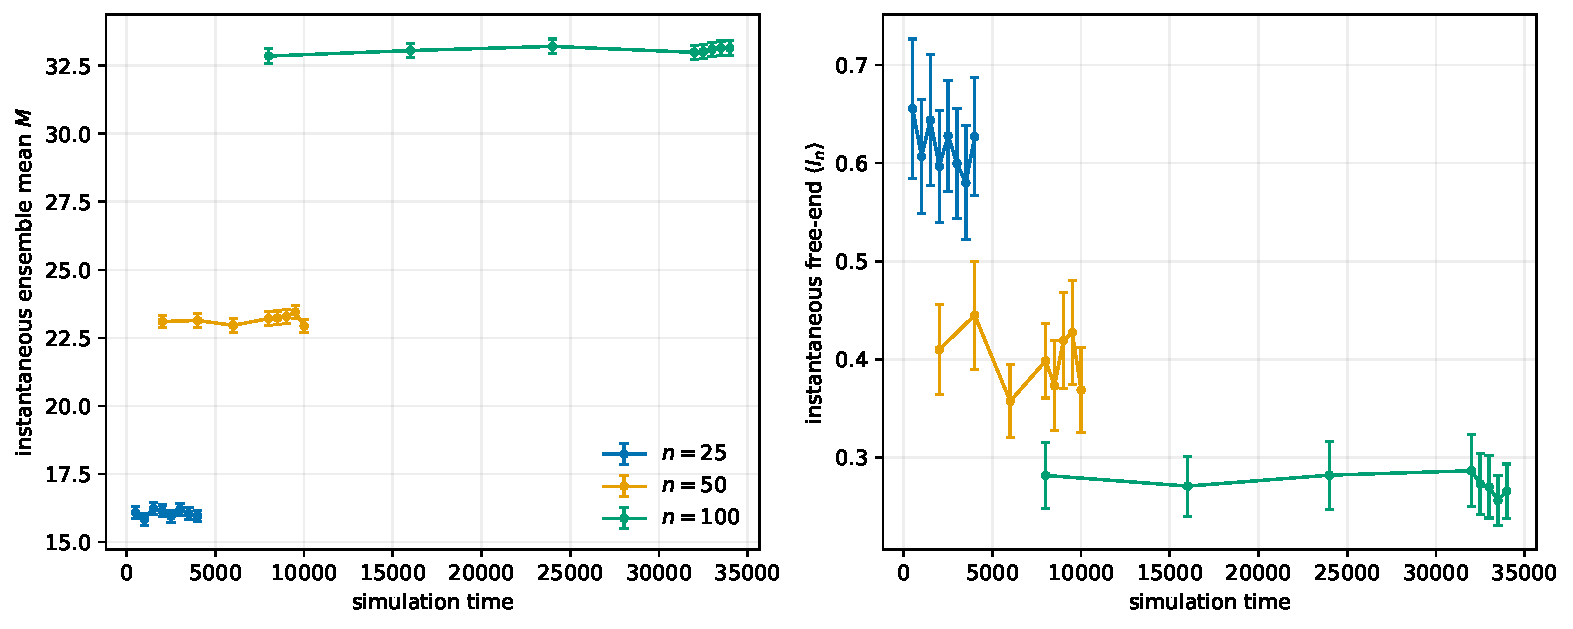
\includegraphics[width=0.88\linewidth]{../figures/open_stationarity_T10.pdf}
\caption{Stationarity diagnostics at left-bath temperature 10: instantaneous total action and free-end action.}
\end{figure}
\begin{figure}[p]
\centering
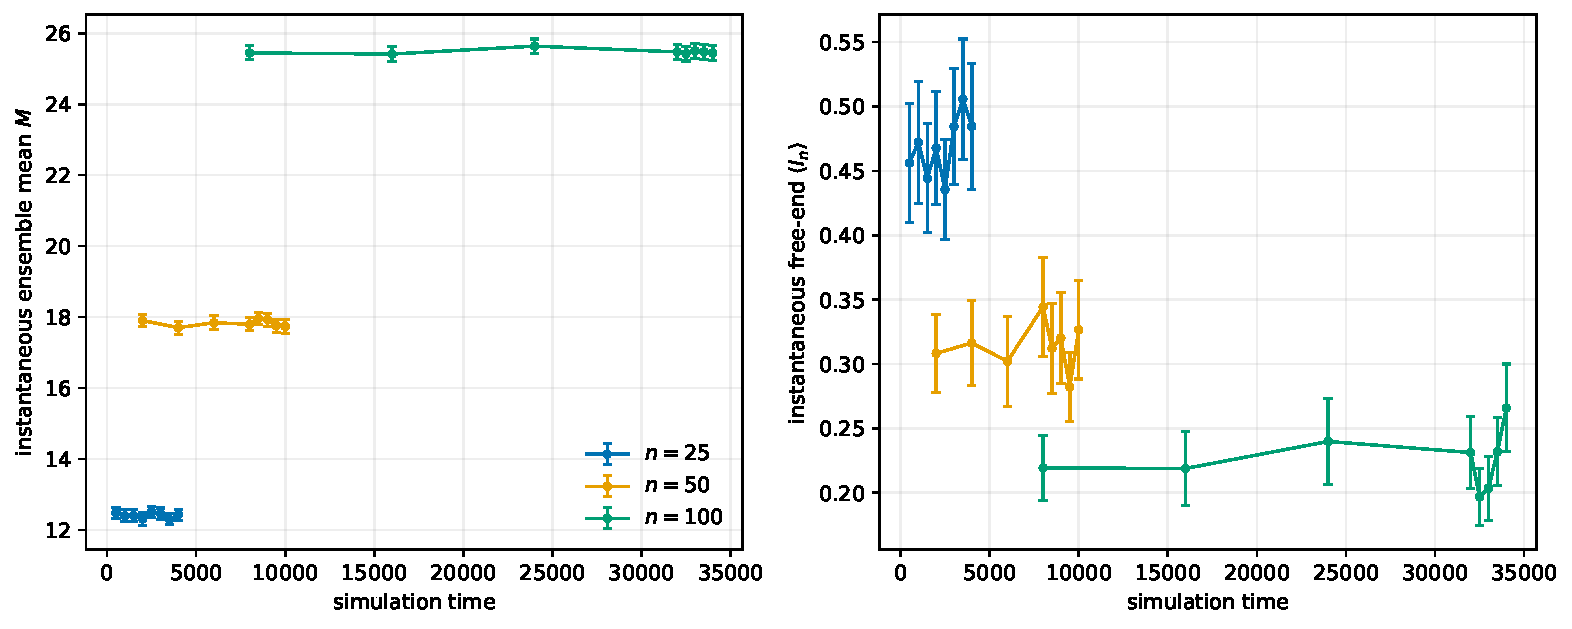
\includegraphics[width=0.88\linewidth]{../figures/open_stationarity_T6.pdf}
\caption{Stationarity diagnostics at left-bath temperature 6: instantaneous total action and free-end action.}
\end{figure}
\begin{figure}[p]
\centering
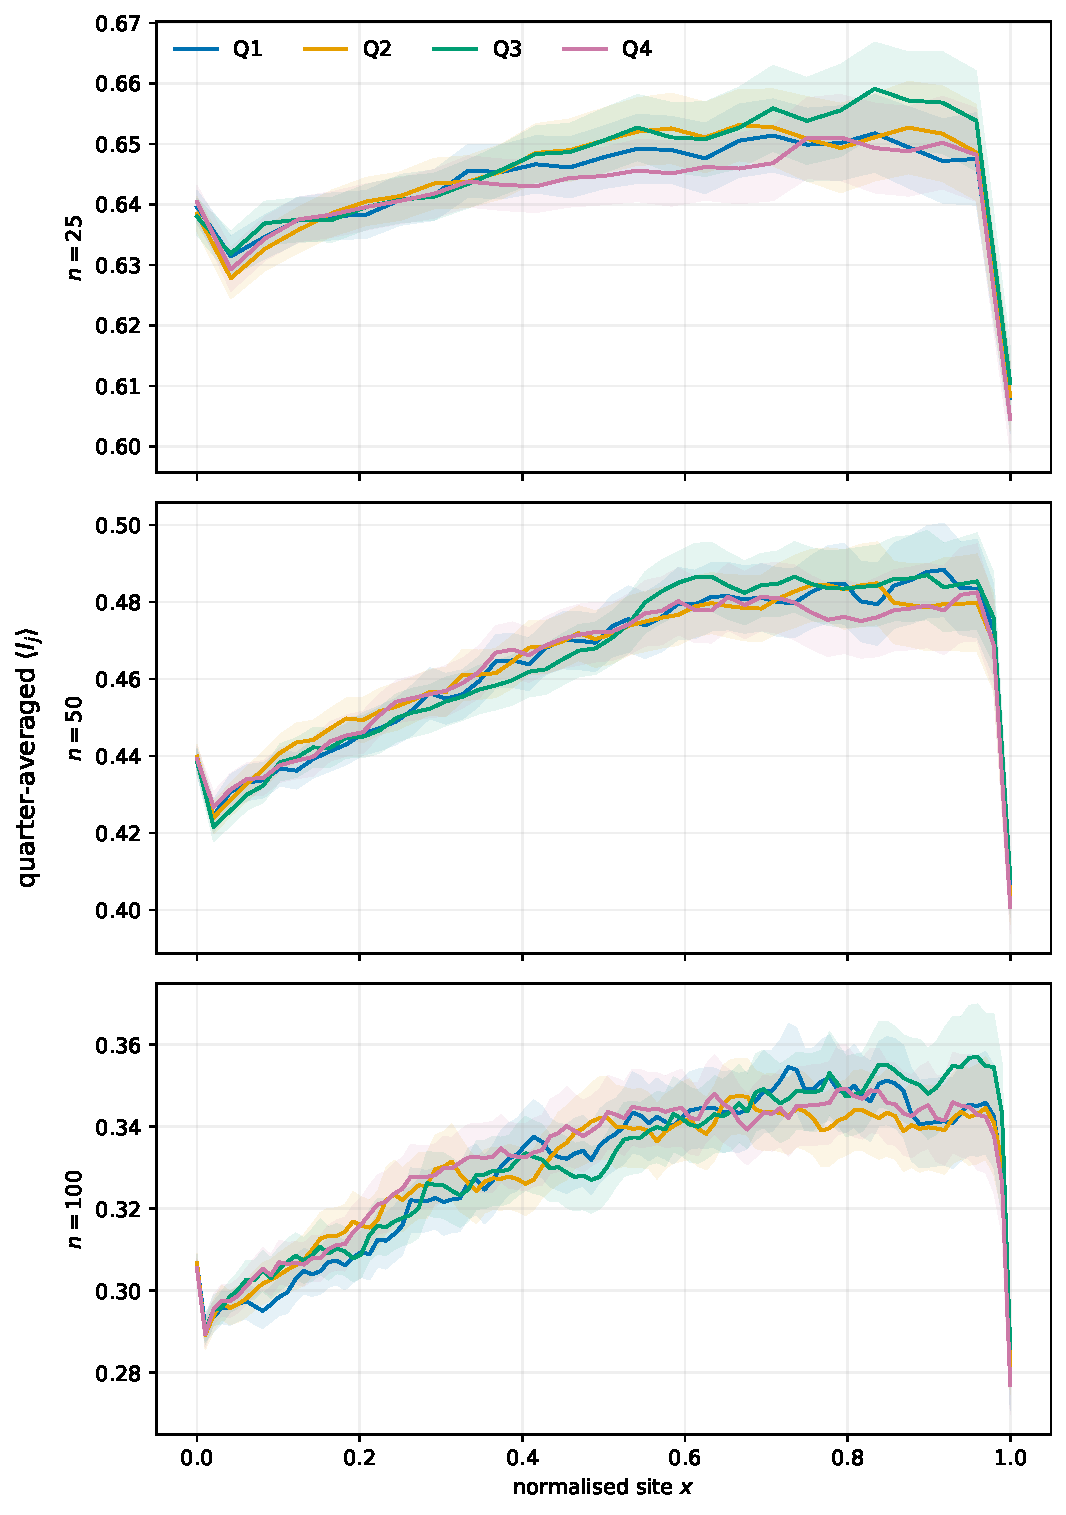
\includegraphics[width=0.88\linewidth]{../figures/open_quarter_profiles_T10.pdf}
\caption{Separate quarter-averaged action profiles at left-bath temperature 10.}
\end{figure}
\begin{figure}[p]
\centering
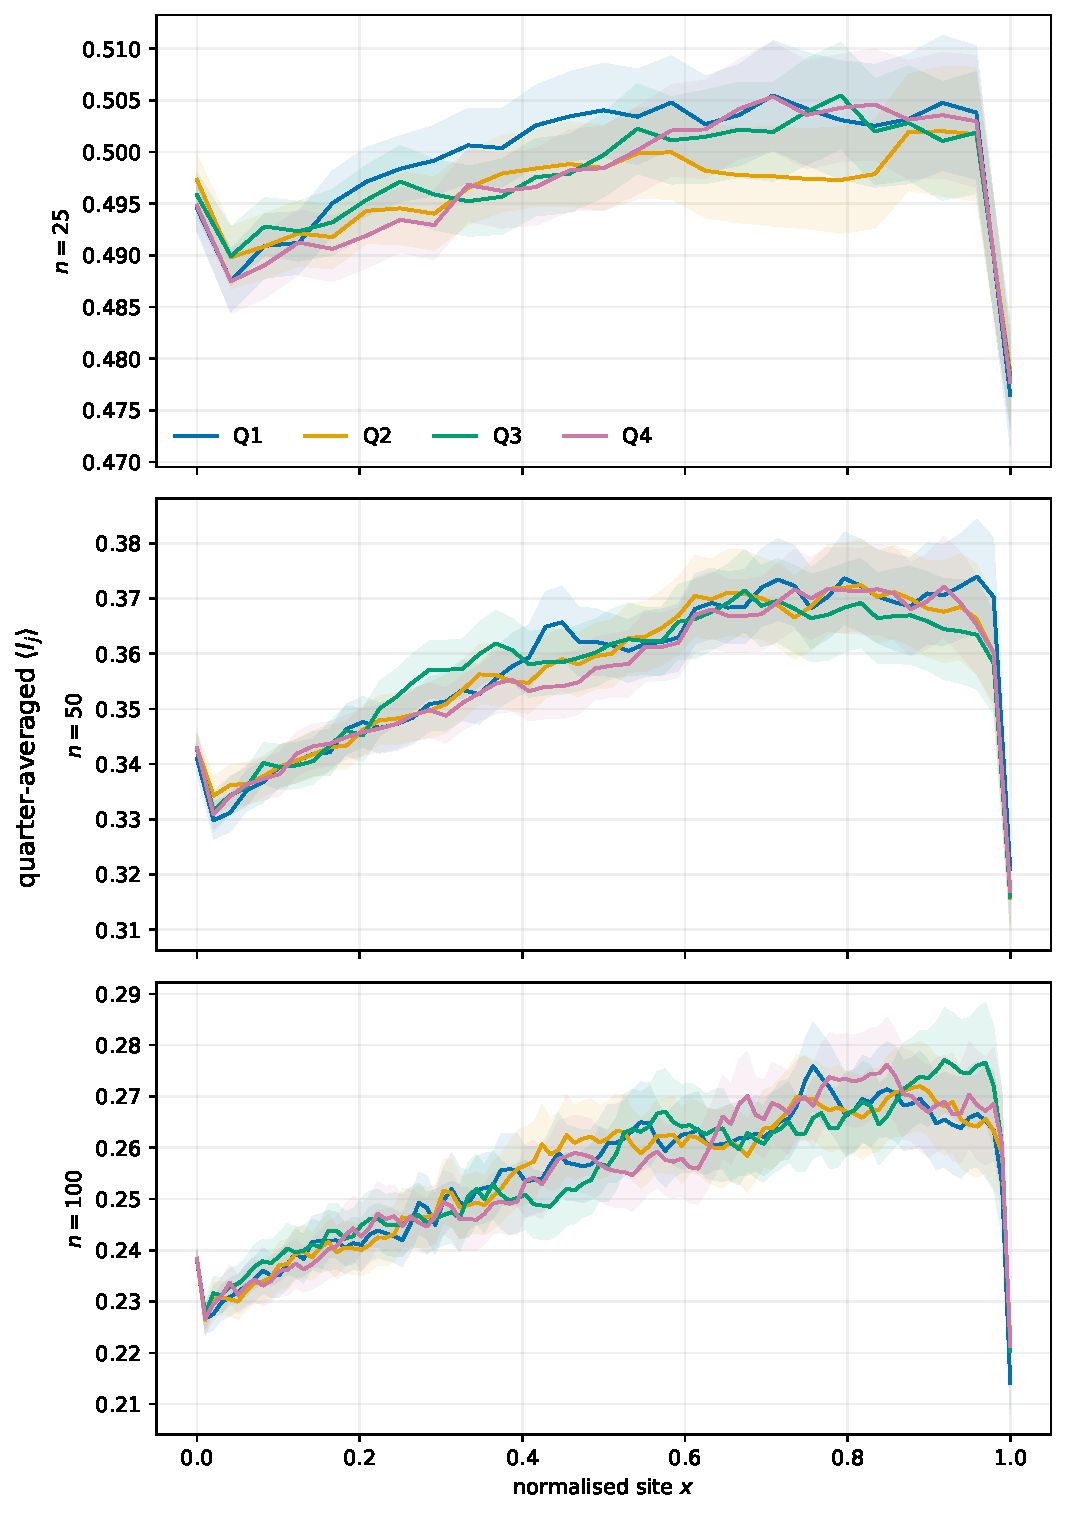
\includegraphics[width=0.88\linewidth]{../figures/open_quarter_profiles_T6.pdf}
\caption{Separate quarter-averaged action profiles at left-bath temperature 6.}
\end{figure}
\begin{figure}[p]
\centering
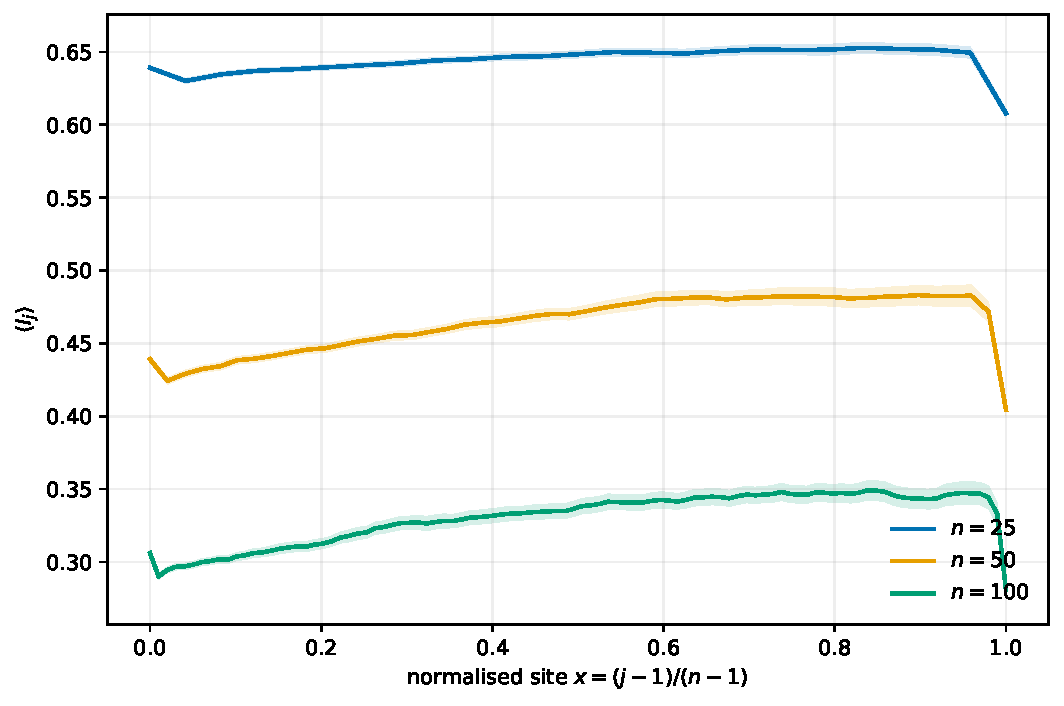
\includegraphics[width=0.88\linewidth]{../figures/open_action_profiles_T10.pdf}
\caption{Raw open-chain action profiles at left-bath temperature 10; bands are pointwise 95 percent intervals.}
\end{figure}
\begin{figure}[p]
\centering
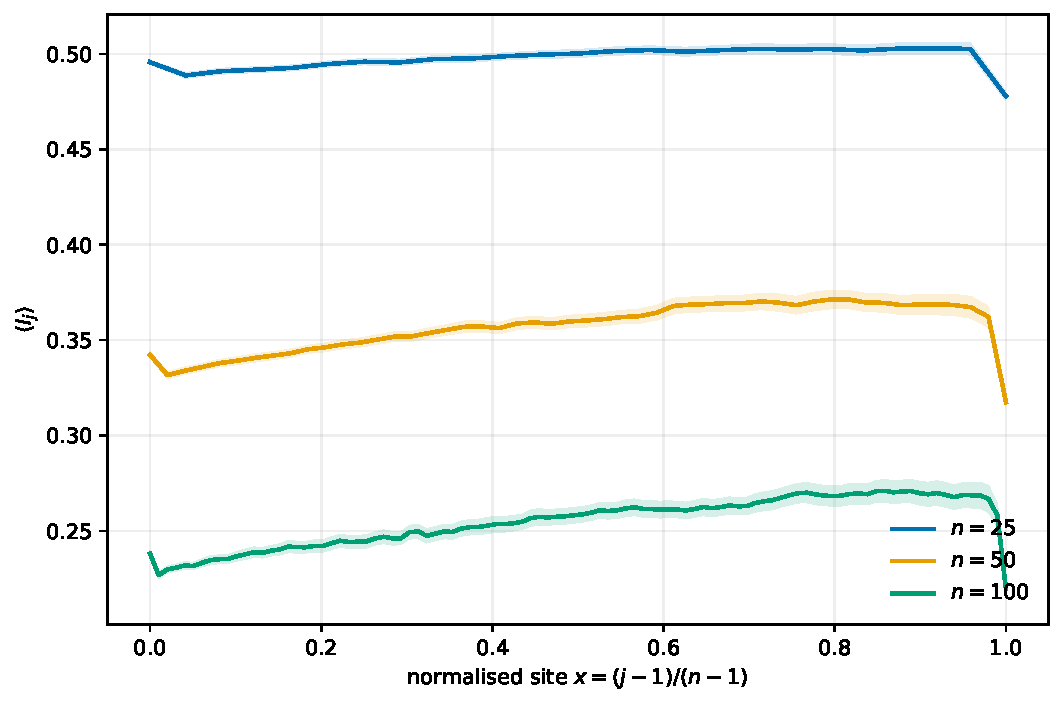
\includegraphics[width=0.88\linewidth]{../figures/open_action_profiles_T6.pdf}
\caption{Raw open-chain action profiles at left-bath temperature 6; bands are pointwise 95 percent intervals.}
\end{figure}
\begin{figure}[p]
\centering
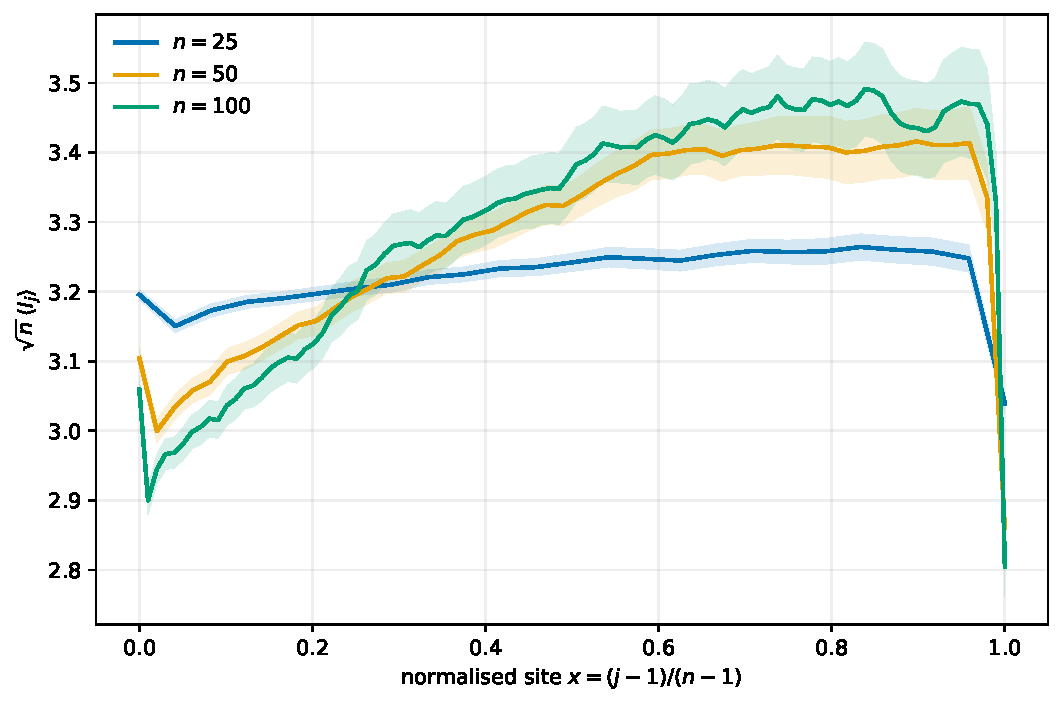
\includegraphics[width=0.88\linewidth]{../figures/open_action_profiles_rescaled_T10.pdf}
\caption{Fixed-exponent collapse test $\sqrt{n}\langle I_j\rangle$ at left-bath temperature 10.}
\end{figure}
\begin{figure}[p]
\centering
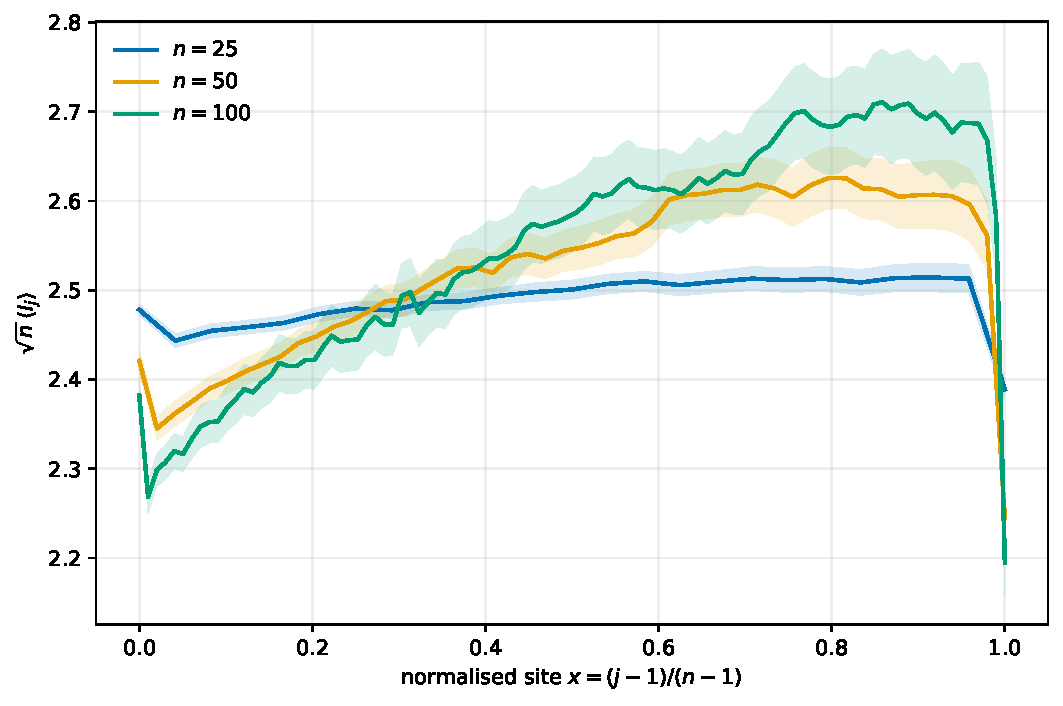
\includegraphics[width=0.88\linewidth]{../figures/open_action_profiles_rescaled_T6.pdf}
\caption{Fixed-exponent collapse test $\sqrt{n}\langle I_j\rangle$ at left-bath temperature 6.}
\end{figure}

\clearpage
\section{Mid-chain and free-end scaling}
\scriptsize
\begin{longtable}{l l r r r r c}
\toprule
$T_L$ & metric & $n$ & site & mean & SE & stationary\\
\midrule
\endfirsthead
T10 & free\_end & 25 & 25 & 0.60781 & 0.00139 & yes \\
T10 & free\_end & 50 & 50 & 0.40444 & 0.00207 & yes \\
T10 & free\_end & 100 & 100 & 0.28052 & 0.00223 & no \\
T10 & mid\_chain & 25 & 13 & 0.64842 & 0.00132 & yes \\
T10 & mid\_chain & 50 & 25 & 0.46997 & 0.00203 & yes \\
T10 & mid\_chain & 100 & 50 & 0.33639 & 0.00268 & no \\
T6 & free\_end & 25 & 25 & 0.47779 & 0.00118 & yes \\
T6 & free\_end & 50 & 50 & 0.31745 & 0.00165 & yes \\
T6 & free\_end & 100 & 100 & 0.21951 & 0.00198 & yes \\
T6 & mid\_chain & 25 & 13 & 0.50016 & 0.00109 & yes \\
T6 & mid\_chain & 50 & 25 & 0.35980 & 0.00167 & yes \\
T6 & mid\_chain & 100 & 50 & 0.25822 & 0.00213 & yes \\
\bottomrule
\end{longtable}

\begin{longtable}{l l r r l r c}
\toprule
$T_L$ & metric & exponent & OLS SE & 95\% CI ($df=1$) & log-SSE & all stationary\\
\midrule
\endfirsthead
T10 & mid\_chain & -0.47339 & 0.00523 & [-0.53982, -0.40696] & 2.62645e-05 & no \\
T10 & free\_end & -0.55776 & 0.01729 & [-0.77748, -0.33804] & 2.87333e-04 & no \\
T6 & mid\_chain & -0.47689 & 9.86565e-04 & [-0.48942, -0.46435] & 9.35260e-07 & yes \\
T6 & free\_end & -0.56105 & 0.01663 & [-0.77239, -0.34971] & 2.65841e-04 & yes \\
\bottomrule
\end{longtable}
\normalsize
Each exponent uses only three chain lengths and therefore has one residual
degree of freedom.  No exponent is adjusted to improve collapse.

\section{Fixed $\sqrt{n}$ collapse}
Profiles are linearly interpolated to the predeclared 101-point grid
$x=0,0.01,\ldots,1$.  Relative spread is
$(\max_n y-\min_n y)/\operatorname{mean}_n y$ and is reported on the full
grid and fixed interior $0.10\le x\le0.90$.

\scriptsize
\begin{longtable}{l l l r r r}
\toprule
$T_L$ & scale & region & grid points & median spread & maximum spread\\
\midrule
\endfirsthead
T10 & raw & full & 101 & 0.6449 & 0.7657 \\
T10 & raw & interior\_0p10\_0p90 & 81 & 0.6406 & 0.7237 \\
T10 & sqrt\_n & full & 101 & 0.0502 & 0.0930 \\
T10 & sqrt\_n & interior\_0p10\_0p90 & 81 & 0.0439 & 0.0671 \\
T6 & raw & full & 101 & 0.6496 & 0.7636 \\
T6 & raw & interior\_0p10\_0p90 & 81 & 0.6481 & 0.7160 \\
T6 & sqrt\_n & full & 101 & 0.0411 & 0.0852 \\
T6 & sqrt\_n & interior\_0p10\_0p90 & 81 & 0.0349 & 0.0758 \\
\bottomrule
\end{longtable}
\normalsize

\section{Penetration depth}
The prospectively fixed threshold is 50 percent of the driven-end action.  The
first raw crossing and its linearly interpolated location are reported without
tail extrapolation.

\scriptsize
\begin{longtable}{l r r r c r r r c}
\toprule
$T_L$ & $n$ & $I_1$ & threshold & reached & first site & interpolated site & site/$n$ & stationary\\
\midrule
\endfirsthead
T10 & 25 & 0.63910 & 0.31955 & no & -- & -- & -- & yes \\
T10 & 50 & 0.43905 & 0.21952 & no & -- & -- & -- & yes \\
T10 & 100 & 0.30599 & 0.15300 & no & -- & -- & -- & no \\
T6 & 25 & 0.49563 & 0.24782 & no & -- & -- & -- & yes \\
T6 & 50 & 0.34236 & 0.17118 & no & -- & -- & -- & yes \\
T6 & 100 & 0.23820 & 0.11910 & no & -- & -- & -- & yes \\
\bottomrule
\end{longtable}
\normalsize

\clearpage
\section{Run-level integrity and provenance}
\scriptsize
\begin{longtable}{r r r r r r r r}
\toprule
$T_L$ & $n$ & seed & threads & valid & nonfinite & projections & seconds\\
\midrule
\endfirsthead
6 & 25 & 2026091425 & 2 & 256 & 0 & 1798104 & 181.94 \\
6 & 25 & 2026091426 & 2 & 256 & 0 & 1796575 & 181.89 \\
6 & 50 & 2026091450 & 2 & 256 & 0 & 6451523 & 820.35 \\
6 & 50 & 2026091451 & 2 & 256 & 0 & 6462082 & 795.44 \\
6 & 100 & 2026091500 & 2 & 256 & 0 & 31351515 & 5089.14 \\
6 & 100 & 2026091501 & 2 & 256 & 0 & 31304163 & 4752.23 \\
10 & 25 & 2026091225 & 2 & 256 & 0 & 2327157 & 193.93 \\
10 & 25 & 2026091226 & 2 & 256 & 0 & 2328091 & 197.19 \\
10 & 50 & 2026091250 & 2 & 256 & 0 & 8403924 & 780.44 \\
10 & 50 & 2026091251 & 2 & 256 & 0 & 8414954 & 778.19 \\
10 & 100 & 2026091300 & 2 & 256 & 0 & 40486534 & 5107.15 \\
10 & 100 & 2026091301 & 2 & 256 & 0 & 40350081 & 4975.42 \\
\bottomrule
\end{longtable}
\normalsize

Parent profile-matrix source SHA-256:
\path{40d13c7547d9c147ca8241ed701e1a1e85540fc0c21db48c4a63a943eccfe3ec}.

Remote freeze commit:
\path{f4b74a06e658478e78b130975b34af20da9d9398}.

Open-chain source SHA-256:
\path{dfee7ed0b416a30f2b27d919c524dfaf37e91ca44312ffbb9d68b7fc1cd36110}.

Binary SHA-256:
\path{09d801e71b7f3bd13cea56aba3d432b471dbf16a726a9866894148a91397575d}.

Analysis SHA-256:
\path{1fd79a163cfccc518cdcfd95064dc994aad32f0854071692a1d00c29fbf69db2}.

Exact commands, seeds, runtimes, complete raw files, merged profiles, separate
quarter profiles, snapshot trajectories, spread curves, and all SHA-256 values
accompany this report.

\end{document}
